%%%%%%%%%%%%%%%%%%%%%%%%%%%%%%%%%%%%%%%%%%%%%%%%%%%%%%%%%%%%%%%%%%
%%%%%%%%%%%%%%%%%%%%%%%%%%%%%%%%%%%%%%%%%%%%%%%%%%%%%%%%%%%%%%%%%%
%Packages
\documentclass[10pt, a4paper]{article}
\usepackage[top=3cm, bottom=4cm, left=1.5cm, right=1.5cm]{geometry}
\usepackage{amsmath,amsthm,amsfonts,amssymb,amscd, fancyhdr, color, comment, graphicx, environ}
\usepackage{float}
\usepackage{mathrsfs}
\usepackage[math-style=ISO]{unicode-math}
\setmathfont{TeX Gyre Termes Math}
\usepackage{lastpage}
\usepackage[dvipsnames]{xcolor}
\usepackage[framemethod=TikZ]{mdframed}
\usepackage{enumerate}
\usepackage[shortlabels]{enumitem}
\usepackage{fancyhdr}
\usepackage{indentfirst}
\usepackage{listings}
\usepackage{sectsty}
\usepackage{thmtools}
\usepackage{shadethm}
\usepackage{hyperref}
\usepackage{setspace}
\hypersetup{
    colorlinks=true,
    linkcolor=blue,
    filecolor=magenta,      
    urlcolor=blue,
}
\usepackage{tcolorbox}
\tcbuselibrary{skins,xparse}

\usepackage{tikz}
\usepackage{subfig}
%%%%%%%%%%%%%%%%%%%%%%%%%%%%%%%%%%%%%%%%%%%%%%%%%%%%%%%%%%%%%%%%%%
%%%%%%%%%%%%%%%%%%%%%%%%%%%%%%%%%%%%%%%%%%%%%%%%%%%%%%%%%%%%%%%%%%
%Environment setup
\mdfsetup{skipabove=\topskip,skipbelow=\topskip}
\newrobustcmd\ExampleText{%
An \textit{inhomogeneous linear} differential equation has the form
\begin{align}
L[v ] = f,
\end{align}
where $L$ is a linear differential operator, $v$ is the dependent
variable, and $f$ is a given non−zero function of the independent
variables alone.
}
\mdfdefinestyle{theoremstyle}{%
linecolor=black,linewidth=1pt,%
frametitlerule=true,%
frametitlebackgroundcolor=gray!20,
innertopmargin=\topskip,
}
\mdtheorem[style=theoremstyle]{Problem}{Exercice}
\newenvironment{Solution}{\textbf{Solution.}}

\definecolor{codegreen}{rgb}{0,0.6,0}
\definecolor{codegray}{rgb}{0.5,0.5,0.5}
\definecolor{codepurple}{rgb}{0.58,0,0.82}
\definecolor{backcolour}{rgb}{0.95,0.95,0.92}

\lstdefinestyle{mystyle}{
    backgroundcolor=\color{backcolour},   
    commentstyle=\color{codegreen},
    keywordstyle=\color{magenta},
    numberstyle=\tiny\color{codegray},
    stringstyle=\color{codepurple},
    basicstyle=\ttfamily\footnotesize,
    breakatwhitespace=false,         
    breaklines=true,                 
    captionpos=b,                    
    keepspaces=true,                 
    numbers=left,                    
    numbersep=5pt,                  
    showspaces=false,                
    showstringspaces=false,
    showtabs=false,                  
    tabsize=2
}

\lstset{style=mystyle}
%%%%%%%%%%%%%%%%%%%%%%%%%%%%%%%%%%%%%%%%%%%%%%%%%%%%%%%%%%%%%%%%%%
%%%%%%%%%%%%%%%%%%%%%%%%%%%%%%%%%%%%%%%%%%%%%%%%%%%%%%%%%%%%%%%%%%
%Fill in the appropriate information below
\newcommand{\norm}[1]{\left\lVert#1\right\rVert}     
\newcommand\course{XXXX0000}                            % <-- course name   
\newcommand\hwnumber{0}                                 % <-- homework number
\newcommand\Information{Someone}                        % <-- personal information
%%%%%%%%%%%%%%%%%%%%%%%%%%%%%%%%%%%%%%%%%%%%%%%%%%%%%%%%%%%%%%%%%%
%%%%%%%%%%%%%%%%%%%%%%%%%%%%%%%%%%%%%%%%%%%%%%%%%%%%%%%%%%%%%%%%%%
%Page setup
\pagestyle{fancy}
\headheight 35pt
\lhead{\today}
\rhead{
\includegraphics[width=0.5cm]{logoF.png}}
\lfoot{}
\pagenumbering{arabic}
\cfoot{\small\thepage}
\rfoot{}
\headsep 1.2em
\renewcommand{\baselinestretch}{1.25}
%%%%%%%%%%%%%%%%%%%%%%%%%%%%%%%%%%%%%%%%%%%%%%%%%%%%%%%%%%%%%%%%%%
%%%%%%%%%%%%%%%%%%%%%%%%%%%%%%%%%%%%%%%%%%%%%%%%%%%%%%%%%%%%%%%%%%
%Add new commands here
\renewcommand{\labelenumi}{\alph{enumi})}
\newcommand{\Z}{\mathbb Z}
\newcommand{\R}{\mathbb R}
\newcommand{\Q}{\mathbb Q}
\newcommand{\NN}{\mathbb N}
\newcommand{\PP}{\mathbb P}
\DeclareMathOperator{\Mod}{Mod} 
\renewcommand\lstlistingname{Algorithm}
\renewcommand\lstlistlistingname{Algorithms}
\def\lstlistingautorefname{Alg.}
\newtheorem*{theorem}{Theorem}
\newtheorem*{lemma}{Lemma}
\newtheorem{case}{Case}
\newcommand{\assign}{:=}
\newcommand{\infixiff}{\text{ iff }}
\newcommand{\nobracket}{}
\newcommand{\backassign}{=:}
\newcommand{\tmmathbf}[1]{\ensuremath{\boldsymbol{#1}}}
\newcommand{\tmop}[1]{\ensuremath{\operatorname{#1}}}
\newcommand{\tmtextbf}[1]{\text{{\bfseries{#1}}}}
\newcommand{\tmtextit}[1]{\text{{\itshape{#1}}}}

\newenvironment{itemizedot}{\begin{itemize} \renewcommand{\labelitemi}{$\bullet$}\renewcommand{\labelitemii}{$\bullet$}\renewcommand{\labelitemiii}{$\bullet$}\renewcommand{\labelitemiv}{$\bullet$}}{\end{itemize}}
\catcode`\<=\active \def<{
\fontencoding{T1}\selectfont\symbol{60}\fontencoding{\encodingdefault}}
\catcode`\>=\active \def>{
\fontencoding{T1}\selectfont\symbol{62}\fontencoding{\encodingdefault}}
\catcode`\<=\active \def<{
\fontencoding{T1}\selectfont\symbol{60}\fontencoding{\encodingdefault}}

%%%%%%%%%%%%%%%%%%%%%%%%%%%%%%%%%%%%%%%%%%%%%%%%%%%%%%%%%%%%%%%%%%
%%%%%%%%%%%%%%%%%%%%%%%%%%%%%%%%%%%%%%%%%%%%%%%%%%%%%%%%%%%%%%%%%%
%Begin now!



\begin{document}

\begin{titlepage}
    \begin{center}
            
        \huge
        \textbf{Ressource 1.03 - Bases de la programmation 1 }
            
        \LARGE
        \textit{Fascicule de travail : TP}
            
        \vspace{1cm}
            \small
        \begin{tabular}{|c|l|}\hline
             Compétence ciblée&  Traiter les données à des fins décisionnelles    \\\hline
             AC couverts&  AC11.05 | Comprendre les structures algorithmiques de base et leur contexte d’usage  \\
             &  – AC11.06 | Prendre conscience de l’intérêt de la programmation   \\ \hline
                & L’objectif de cette ressource est d’acquérir les principes de base de la programmation dans  \\
               Description & un langage de script. Contenus :\\
                &– Structures de données : variables simples et structurées.\\
                & – Structures de contrôles : alternatives et boucles.\\
                & – Lecture et écriture de fichiers.\\
                & On profitera des enseignements pour présenter les bonnes pratiques dans la programmation \\
                &(nommage des variables et des
fonctions, indentation, syntaxe, tests, commentaires, documentations...) \\
                &Cette ressource présente les éléments, concepts et principes de base de la programmation\\
                &  dont la maitrise est indispensable dans l’acquisition de la compétence.  \\
                \hline Mots clés &Programmation – langage\\\hline
                Heures formation&30h\\\hline
                Contrôle Ecrit &1h30 (coefficient 50\%)\\\hline
                Contrôle Pratique &1h (coefficient 50\%)\\\hline
                Semestre&Semestre 1\\\hline
                Vos contacts&\textbf{Mohammed Azerkane}, chargé de TPs : \url{azerkane.m@gmail.com}
\\
                &\textbf{Dorine Tabary}, responsable de l'UE : \url{dorine.tabary@univ-fcomte.fr}
\\\hline
        \end{tabular}




    \vspace{1cm}

\begin{center}
  \noindent\rule{4cm}{0.6pt}  Organisation des séances de TP   \noindent\rule{4cm}{0.4pt}  
    
\end{center}
        \begin{tabular}{|c|l|}\hline
             semaine 39& Premiers programmes   \\\hline
             semaine 40& Les structures de contrôle   \\\hline
             semaine 41& Lecture/ écriture de fichier  \\\hline
             semaine 42& Exemple de sujet de contrôle  \\\hline
        \end{tabular}

    \vspace{0.5cm}
        
    \noindent\rule{12cm}{0.6pt}
        \vfill
        
\includegraphics[width=0.4\textwidth]{logo.png}
        \\            
    \end{center}  
\end{titlepage}




%%%%%%%%%%%%%%%%%%%%%%%%%%%%%%%%%%%%%%%%%%%%%%%%%%%%%%%%%%%%%%%%%%
%%%%%%%%%%%%%%%%%%%%%%%%%%%%%%%%%%%%%%%%%%%%%%%%%%%%%%%%%%%%%%%%%%
%Start the assignment now
%%%%%%%%%%%%%%%%%%%%%%%%%%%%%%%%%%%%%%%%%%%%%%%%%%%%%%%%%%%%%%%%%%
%New problem

%%%%%%%%%%%%%%%%%%%%%%%%%%%%%%%%%%%%%%%%%%%%%%%%%%%%%%%%%%%%%%%%%%
%%%%%%%%%%%%%%%%%%%%%%%%%%%%%%%%%%%%%%%%%%%%%%%%%%%%%%%%%%%%%%%%%%
%Start the assignment now
%%%%%%%%%%%%%%%%%%%%%%%%%%%%%%%%%%%%%%%%%%%%%%%%%%%%%%%%%%%%%%%%%%
%New problem



\newpage



\begin{tcolorbox}[lefttitle=2cm, colframe=gray!75!black, title= \textbf{Examen des connaissances pratiques}]
Comment se passera l'examen ?
L'examen sera tiré de sujets d'advent of code\footnote{\url{https://adventofcode.com/} }.

Seront pris en compte les commentaires, et le respect des règles de bon codage.

\end{tcolorbox}

\begin{tcolorbox}[lefttitle=2cm, colframe=gray!75!black, title= \textbf{Les Travaux Pratiques}]

L'objectif est d'acquérir les notions de base de la programmation Python.

Des corrections sont disponibles sur le git.

Il est donc contre productif de copier directement les solutions sur internet ou d'utiliser un LLM (vous aurez tout le loisir les années suivantes d'en manipuler).

Lors de chaque TP, les premiers exercices non optionnels doivent être réalisés. 
La partie optionnelle concerne les plus aguerris d'entre vous.
Pour ces derneirs, le jeu est d'aller le plus loin possible dans le temps imparti.

Il est également obligatoire à la fin de chaque TP, de compléter la partie BILAN.

\end{tcolorbox}



\begin{tcolorbox}[lefttitle=2cm, colframe=gray!75!black, title= \textbf{Evénements}]
Il existe plusieurs événements informatiques.


\paragraph{Nuit de l'info.}

\textbf{Date} : 7 et 8 décembre 2023, de 16h38 à 08h06. En présentiel.

\textbf{Détails} : Un serious-game regroupant des milliers d’étudiants pour développer une application informatique en une nuit. L'événement a lieu dans l'université de Besançon (route de gray, bâtiment C) et se déroule par équipe.

\textbf{Contact} : Mme Tabary (membre de l'équipe organisatrice)



\paragraph{Global Game Jam.}

\textbf{Date} : mi-janvier 2024. En présentiel avec possibilité de distanciel.

\textbf{Détails} : L'évènement se déroule en 48 heures, pendant lesquelles les développeurs doivent concevoir un jeu-vidéo à partir d'un thème partagé par tous les participants. Leurs créations sont ensuite qualifiées par un jury. L'événement a lieu dans l'université de Besançon (maison des étudiants) et se déroule par équipe.

\textbf{Contact} : Mme Tabary  (participante, ou membre de l'équipe organisatrice si pénurie)


\paragraph{Advent of code.}

\textbf{Date} : 1 - 25 décembre 2023. En distanciel.

\textbf{Détails} : L'Advent of Code (\url{https://adventofcode.com/}) est une série annuelle de défis de programmation informatique qui suit un calendrier de l'Avent.

Les énigmes (puzzles) de programmation couvrent un vaste champ de compétences et peuvent être résolues en utilisant n'importe quel langage de programmation. Les participants s'affrontent également en fonction de leur vitesse dans les classements mondiaux et privés.  En individuel.

\textbf{Contact} :  Mme Tabary  (participante), avec possibilité de s'incruster dans un groupe privé.


\end{tcolorbox}
\begin{tcolorbox}[lefttitle=2cm, colframe=gray!75!black, title= \textbf{Le manuel}]
\url{https://docs.python.org/fr/3/contents.html}
\end{tcolorbox}

\newpage
\setcounter{tocdepth}{2}
\tableofcontents 

\newpage

\section{TP1 : Premiers programmes}


\subsection{Installer et configurer Python}
\textit{(Inutile avec les ordinateurs de l'université, déjà configurés).}


Python est un \textbf{langage interprété}. Contrairement au langage compilé qui fournit un code binaire utilisable et réutilable par la machine, le langage interprété nécessite d'utiliser un interpréteur à chaque exécution.


\begin{figure}[H]
\begin{minipage}[b]{0.4\textwidth}

    \begin{tikzpicture}
\node (cs) at (0,1) {\textcolor{blue}{Code source}};
\node[draw, fill=blue!20!white] (comp) at (0,0) {Compilateur};
\node (cb) at (0,-1) {Code binaire};
\node[draw, fill=blue!20!white] (se) at (4,-1) {Système d'exploitation};
\node (entree) at (4,0) {\textbf{Entrée(s)}};
\node (sortie) at (4,-2) {\textbf{Sortie}};


\draw[-latex] (cs) -- (comp) ;
\draw[-latex] (comp) -- (cb);
\draw[-latex] (cb) -- (se);
\draw[-latex] (entree) -- (se);
\draw[-latex] (se) -- (sortie);

\end{tikzpicture}  
\caption{Langage compilé}

\end{minipage}\hfill
\begin{minipage}[b]{0.4\textwidth}
\begin{tikzpicture}
\node (cs) at (0,1) {\textcolor{blue}{Code source} };
\node[draw, fill=blue!20!white] (int) at (4,-1) {Interpréteur};
\node (entree) at (4,0) {\textbf{Entrée(s)}};
\node (sortie) at (4,-2) {\textbf{Sortie}};


\draw[-latex,-](cs) -- (0,-1);
\draw[-latex] (0,-1) --(int);
\draw[-latex] (entree) -- (se);
\draw[-latex] (se) -- (sortie);

\end{tikzpicture}  
    \caption{Langage interpreté}
    \label{fig:com}
\end{minipage}
\end{figure}


Avant l'installation, n'oubliez pas de vérifier que Python est bien présent de votre ordinateur.


Une aide à l'installation est disponible sous ce lien :
\url{https://www.commentcoder.com/installer-python/}

Vos professeurs peuvent également vous aider pour installer l'environnement de travail sur votre machine personnelle (très recommandé).

\subsection{Rangement de votre espace de travail}
Tous vos programmes devront être rangés dans des dossiers.
Par exemple, enregistrez votre programme dans un dossier Cours, dans un dossier Semestre 1, dans un dossier Bases de la programmation, dans un dossier tp1.

\subsection{Echauffement}



\subsubsection{Ecrire et lire sur un terminal de commande}


\paragraph{Sortie écran}
Pour afficher une chaîne de caractères en Python 3, ouvrez un éditeur de texte et
écrivez :

\lstinputlisting[language = python]{chapitre1/codes/premier.py}


\begin{enumerate}
    \item Enregistrez ce dossier sous le nom de premier.py
    \item Dans le terminal, exécuter : python3 premier.py
\end{enumerate}

Avec le terminal de commande, allez dans le dossier contenant votre programme.

    \begin{figure}[H]
    \centering
    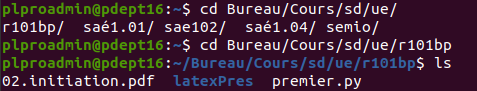
\includegraphics[scale = 0.7]{chapitre1/figures/premier.png}
    \caption{Commandes pour se déplacer dans la hiérarchie de fichiers.}
    \label{fig:enter-label}
\end{figure}

Exécutez le programme avec l'instruction python3 premier.py.

\begin{figure}[H]
    \centering
    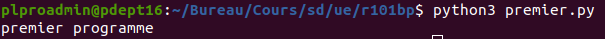
\includegraphics[scale = 0.7]{chapitre1/figures/premier2.png}
    \caption{Commande pour  exécuter un programme.}
\end{figure}



\begin{tcolorbox}[lefttitle=2cm, colframe=gray!75!black, title= \textbf{Exercices}]
A partir du programme premier.py, écrivez les programmes suivant :Exercice


\textbf{1$\diamondsuit$-}
Ecrire le programme  qui ne prend rien en entrée et donne en sortie le texte suivant.
\begin{figure}[H]
    \centering
    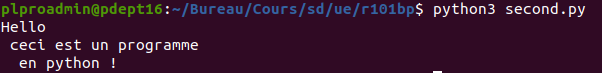
\includegraphics[scale=0.6]{chapitre1/figures/second.png}
\end{figure}
\textbf{2$\diamondsuit$-}
Sauriez-vous le faire en n'utilisant qu'une seule fois l'instruction print ?
\end{tcolorbox}

\paragraph{Entrée utilisateur}


Pour entrer une chaîne de caractères en Python 3, ouvrez un éditeur de texte et
écrivez :

\lstinputlisting[language = python]{chapitre1/codes/programmeAvecEntrees.py}



La sortie écran obtenue est la suivante : 

\begin{figure}[H]
    \centering
    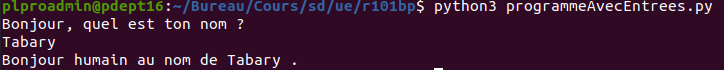
\includegraphics[scale = 0.7]{chapitre1/figures/entree.png}
\end{figure}

\begin{tcolorbox}[lefttitle=2cm, colframe=gray!75!blue, title= \textbf{Tip for Code 1 : "\textit{code is read much more often than it is written}", Guido van Rossum}]


Commentez un paragraphe avec : """.

Commentez une ligne avec : \#.

\textbf{Et quand vous codez, rajoutez des commentaires.}

\url{https://peps.python.org/pep-0008/}

\end{tcolorbox}


\begin{tcolorbox}[lefttitle=2cm, colframe=gray!75!black, title= \textbf{Exercices}]
\textbf{1$\diamondsuit$-}
Ecrire le programme qui donne en sortie le texte suivant.
\begin{figure}[H]
    \centering
    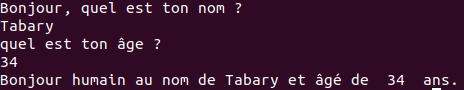
\includegraphics[scale=0.6]{chapitre1/figures/entree2.png}
\end{figure}
\textbf{2$\diamondsuit~\diamondsuit$-}
Modifiez le programme afin d'afficher en plus l'année de naissance.
\begin{figure}[H]
    \centering
    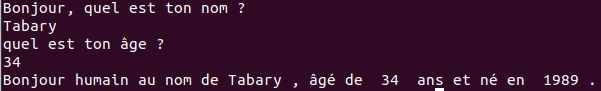
\includegraphics[scale=0.6]{chapitre1/figures/entree3.png}
\end{figure}


\textbf{Aide} : Tip for Code 2 

\textbf{3$\diamondsuit~\diamondsuit~\diamondsuit$ (optionnel)-}
On suppose en plus que la taille est demandée.
L'utilisateur entre un texte qui peut être selon les formats suivants : 177.56cm, ou 177cm, ou 17756cm.
Le terminal répond dans tous les cas :
\begin{figure}[H]
    \centering
    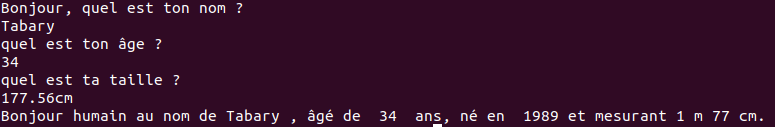
\includegraphics[scale=0.6]{chapitre1/figures/entree4.png}
\end{figure}
\textbf{Aide} : Tip for Code 2 (encore)

\end{tcolorbox}

\begin{tcolorbox}[lefttitle=2cm, colframe=gray!75!blue, title= \textbf{Tip for Code 2 : "\textit{Le shell est votre ami}"}]
Les bugs, ou erreurs de programmation, sont inévitables dans le développement de logiciels complexes, même pour les programmeurs les plus expérimentés.
Il faut savoir lire le code erreur associé.

Une erreur qui risque d'apparaître dans votre cas est la suivante :
\begin{figure}[H]
    \centering
    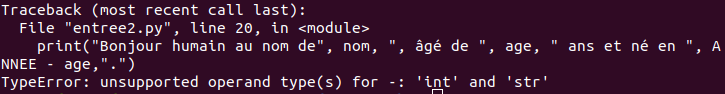
\includegraphics[scale=0.6]{chapitre1/figures/entreeErr.png}
\end{figure}

Dans ce cas, l'erreur se situe \textbf{ligne 20}.

Une variable de type string (texte) est utilisée à la place d'une variable de type int (entier).

En effet ANNEE est une variable globale de type entier (int).
Or, il est impossible de soustraire un texte d'un entier.
Il faut donc changer le type de la variable age afin qu'elle soit un entier.
Cette démarche s'appelle le transtypage.
Pour ce faire, vous pouvez écrire : (int)age.

Source : \url{https://docs.python.org/fr/3/tutorial/inputoutput.html}

\end{tcolorbox}
\subsubsection{Les conditionnelles}
Maintenant, l'objectif est de maîtriser l'alternative\footnote{ \url{https://docs.python.org/fr/3/tutorial/controlflow.html\#if-statements}}.
Testez le programme suivant en respectant bien les indentations.



\lstinputlisting[language = python]{chapitre1/codes/conditionnelle.py}


\begin{tcolorbox}[lefttitle=2cm, colframe=gray!75!blue, title= \textbf{Tip for Code 3 : Indentations et espaces}]

Les annotations pour les variables doivent comporter un seul espace après les deux points.
    Il ne doit pas y avoir d'espace avant les deux points (voir ligne 17).
    Si une affectation a un côté droit, le signe d'égalité doit avoir exactement un espace des deux côtés (voir ligne 11).

Source : Variable Annotations de \url{https://peps.python.org/pep-0008/}

la commande typeof(maVariable) permet de récupérer le type de la variable.

\end{tcolorbox}

\begin{tcolorbox}[lefttitle=2cm, colframe=gray!75!black, title= \textbf{Exercices}]
\textbf{1$\diamondsuit$-}
Ecrire le programme qui spécifie si la personne est mineur, majeure, ou est dans l'année de sa majorité.
\textbf{2$\diamondsuit$-}
Modifier le programme pour incorporer une variale etat qui prend la valeur "mineur", "majeure", ou "est dans l'année de sa majorité", selon l'âge de entrée par l'utilisateur.

\end{tcolorbox}


\subsubsection{Les itératives}
\paragraph{boucle for}
Maintenant, l'objectif est de travailler la boucle for\footnote{ \url{https://docs.python.org/fr/3/reference/compound_stmts.html\#the-while-statement}}.
Testez le programme suivant en respectant bien les indentations.
\lstinputlisting[language = python]{chapitre1/codes/tab.py}

\begin{tcolorbox}[lefttitle=2cm, colframe=gray!75!black, title= \textbf{Exercices}]

\textbf{1$\diamondsuit$-}
Modifier le programme pour incorporer la question pour chaque étudiant "L'étudiant est il venu en cours ? (n/y)".
Si la réponse est "n", alors le prénom de l'étudiant est rajouté à une liste d'étudiants absents.

Ensuite afficher la nouvelle liste des étudiants absents.

\begin{figure}[H]
    \centering
    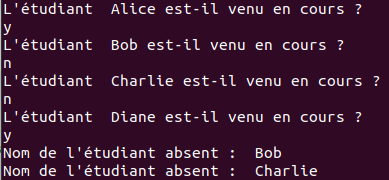
\includegraphics[scale=0.6]{chapitre1/figures/for.png}
\end{figure}
\textit{(optionnel) Quel est, selon la taille de la liste d'entrée, le nombre d'opérations du programme ?}


\textbf{(optionnel) 2$\diamondsuit~\diamondsuit$-}
Réaliser un programme vérifiant qu'aucun étudiant n'est en double dans le tableau.

\textit{ Quel est, selon la taille de la liste d'entrée, le nombre d'opérations du programme ?}

\end{tcolorbox}

\paragraph{Boucle while}
Maintenant, l'objectif est de travailler avec la boucle while\footnote{ \url{https://docs.python.org/fr/3/reference/compound_stmts.html\#the-while-statement}}.

Ce programme modifie le programme précédent afin de s'assurer que l'entrée utilisateur est correcte.
Implémentez-le.
\lstinputlisting[language = python]{chapitre1/codes/while.py}

\begin{tcolorbox}[lefttitle=2cm, colframe=gray!75!black, title= \textbf{Exercices}]

\textbf{1$\diamondsuit$-}
Modifier le programme pour demander si le prénom de l'étudiant présent est bien orthographié.

\textbf{(optionnel)2$\diamondsuit~\diamondsuit~\diamondsuit$-}
Continuer le programme afin de demander une confirmation de l'orthographe avant de valider le prénom.
Modifier le prénom dans la liste s'il était mal orthographié.

\end{tcolorbox}


\subsection{Le juste prix}
Réaliser ce programme :

Un prix caractérisé par une variable globale est déjà présent dans le programme (variable globale). Le but pour l’utilisateur est de deviner ce prix. Chaque fois que l’utilisateur se trompe, l’ordinateur lui dit si c’est plus ou moins que le prix qu’il a donné. Le joueur a gagné une fois qu'il a trouvé le bon prix. Un compteur d'essai donne le nombre de coups nécessaire pour trouver ce juste prix.

\textit{(Optionnel) A votre avis, quelle stratégie de jeu est la meilleure ? et pourquoi sa complexité est de $log (n)$, avec $n$ la taille de la liste ?}


\subsubsection{Réaliser ce programme}

\subsubsection{(Optionnel) Variantes du juste prix}
\paragraph{En entrée, prendre une variable de type entier issue de la librairie random}
\paragraph{En entrée, prendre une voyelle aléatoire (toujours avec la librairie random)}
\paragraph{Avec un nombre de coups limité} Le nombre de coups est défini avec une variable globale.
\paragraph{De faire jouer deux joueurs.} Chacun choisit une lettre de l'alphabet. Le plus rapide à la trouver a gagné.
\paragraph{De faire jouer x joueurs entre eux.} Chacun choisit une lettre de l'alphabet. Le plus rapide à la trouver a gagné. 

\subsubsection{(Optionnel) Générateur des nombres de la suite de Fibonacci}
Sans utiliser de sous-fonction, faite un générateur des nombres de la suite de Fibonacci\footnote{https://fr.wikipedia.org/wiki/Suite\_de\_Fibonacci}.

\newpage

\subsection{Bilan (obligatoire)}



\makebox[0.75\textwidth]{Lors de ce TP, vous vous êtes arrêté à quel exercice ? \enspace\hrulefill}


\makebox[1\textwidth]{Remplir le tableau}

\textbf{Partie savoir faire}
\begin{itemize}
    \item Niveau 1 : Je n'ai pas su l'implémenter. C'est du charabiah pour moi. 
    \item Niveau 2 : J'ai lu le sujet. Les couleurs sont jolies. J'ai fini le premier exercice les yeux rivés sur mon clavier pour chercher les touches. Les erreurs de l'interpréteur me semblent incompréhensibles.
    \item Niveau 3 : J'ai pu avancer à la moitié du sujet, même si c'est difficile et que l'ordi est farceur (comme tous les ordis). Je prends beaucoup de temps à comprendre les erreurs du shell, mais j'y arrive !
    \item Niveau 4 : J'ai complété le TP avec aisance. La plupart des erreurs du shell me sont compréhensibles.
    \item Niveau 5 : J'ai complété le TP, exercices optionnels compris ! J'ai une grande agilité\footnote{agilité $\rightarrow$ ne pas utiliser la souris en codant} quand je code. 
\end{itemize}


\textbf{Partie savoir être}
\begin{itemize}
    \item Niveau 1 :  Pour finir au plus vite, j'élabore des stratégies (copier directement la réponse ou chercher à camoufler le désintérêt : "Si je n'y arrive pas, c'est que le prof n'est pas venu assez vite me donner la solution"). 
    \item Niveau 2 : L'objectif est d'avoir la moyenne sans trop y laisser du temps ou de l'énergie. Je suis bien obligé de faire le TP, même si l'idée de me servir du pannel de ressources me semble saugrenue. Si c'est possible de récupérer la réponse (ou de suivre à côté d'un camarade\footnote{Mais si, c'est du travail d'équipe : il code et je le soutiens émotionnellement !}), alors je ne dirai pas non. 
    \item Niveau 3 : Je prends doucement mes marques. Je me suis servi de façon hésitante de plusieurs ressoures dispos (shell, camarades, enseignants, manuel, sites web, ou même canard\footnote{\url{https://fr.wikipedia.org/wiki/M\%C3\%A9thode_du_canard_en_plastique}}) en cherchant à comprendre leur réponse. J'aimerais un jour pouvoir développer  mes propres projets et il faut pour cela que je gagne en autonomie.
    \item Niveau 4 :   Je suis autonome dans l'utilisation des ressoures disponibles (shell, camarades, enseignants, manuel, sites web, ou même canard\footnotemark[7]). J'ai même un projet personnel en cours que j'aimerais finir.
    \item Niveau 5 : J'évolue avec aisance dans cet environnement ! Je  fais même partie dorénavant des ressoures dispos et  j'échange facilement sur ces notions. J'ai plusieurs projets informatiques personnels. 
\end{itemize}

\begin{table}[H]
    \centering
    \begin{tabular}{|c|c|c|} \hline
        \textbf{Notions} & \textbf{Niveau atteint} (de 1 à 5) \textbf{Savoir faire}  & \textbf{Niveau atteint} (de 1 à 5) \textbf{Savoir être}\\\hline
        Instructions simples & & \\\hline
        Variables &&\\\hline
        Conditionnelles &&\\\hline
        Boucle For &&\\\hline
        Boucle While && \\\hline
        Respect des règles de bon codage && \\\hline
    \end{tabular}
\end{table}



\begin{tcolorbox}[lefttitle=2cm, colframe=gray!75!green, title= \textbf{SUPER TIP}]

Pour finir, un site pour s'entraîner/tester les instructions. En français.

Source : \url{https://www.geeksforgeeks.org/python-tuples/?ref=lbp}
\end{tcolorbox}






\newpage
\section{TP2 : Les structures de données}

    La liste est une collection ordonnée et modifiable. Elle autorise la duplication des items.
    
    Le tuple est une collection ordonnée et immuable. Permet la duplication des items.
    
    Set est une collection non ordonnée, non modifiable et non indexée. Pas d'items en double.
    
    Dictionnaire : collection ordonnée et modifiable. Pas d'items en double.
\subsection{Lists}

\textbf{Les éléments de la liste sont ordonnés, modifiables et peuvent être dupliqués.}

Pour manipuler une liste, ouvrez un éditeur de texte et
écrivez :

\lstinputlisting[language = python]{chapitre2/codes/liste.py}

La sortie écran obtenue est la suivante : 

\begin{figure}[H]
    \centering
    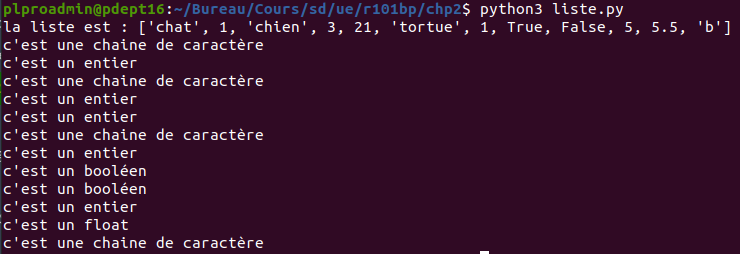
\includegraphics[scale = 0.7]{chapitre2/figures/liste1.png}
\end{figure}

\begin{tcolorbox}[lefttitle=2cm, colframe=gray!75!blue, title= \textbf{Tip for Code 1 : "\textit{Pour un code svelte et en bonne santé}"}]

Votre code commence à prendre de la place.

Par convention, la largeur maximale d'une ligne est de 79 charactères.

Le caractère $\backslash$ permet de couper des lignes trop longues. 

\url{https://peps.python.org/pep-0008/#maximum-line-length}

\end{tcolorbox}


\begin{tcolorbox}[lefttitle=2cm, colframe=gray!75!black, title= \textbf{Exercices}]
\textbf{1$\diamondsuit$-}
Complétez le programme suivant de façon à affecter trois listes : listeChaine, listeBool, listeInt, listeFloat, et listeAutres.
Afficher ces listes de façon à générer la sortie terminale suivante.

\begin{figure}[H]
    \centering
    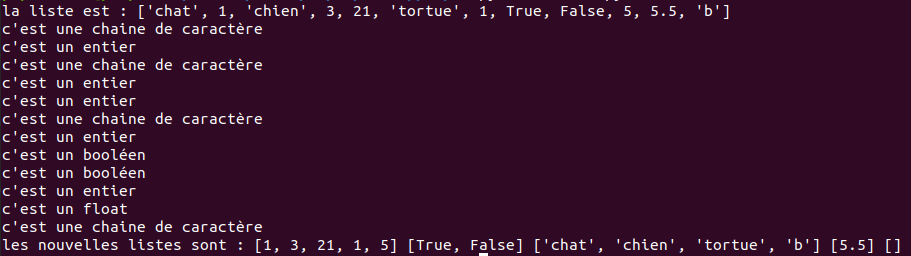
\includegraphics[scale=0.47]{chapitre2/figures/liste2.png}
\end{figure}


\textbf{2$\diamondsuit$-}
Modifiez le programme afin de ranger par ordre croissant listeEntier.

Modifiez le programme afin d'inverser listeChaine.

\textbf{Aide} : \url{https://www.w3schools.com/python/python_lists_methods.asp}

\textbf{(optionnel)3$\diamondsuit~\diamondsuit$-}
Modifiez le programme afin d'afficher une liste qui contient l'avant-dernier éléments de chacune des listes (ou rien si la liste est plus petite).

Et afficher une valeur au hasard de cette liste.

\textbf{Aide} : random.choice(maListe) \url{https://docs.python.org/3/library/random.html}


\end{tcolorbox}

\subsubsection{Strings}

Les strings sont des listes un peu particulières\footnote{\url{https://www.w3schools.com/python/python_strings_methods.asp}}.

Ouvrez un éditeur de texte et écrivez :

\lstinputlisting[language = python]{chapitre2/codes/string.py}

La sortie écran que vous devez obtenir est la suivante : 

\begin{figure}[H]
    \centering
    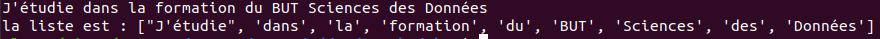
\includegraphics[scale = 0.5]{chapitre2/figures/string.png}
\end{figure}

\begin{tcolorbox}[lefttitle=2cm, colframe=gray!75!blue, title= \textbf{Tip for Code 2 : "\textit{Les expressions régulières}"}]

\begin{figure}[H]
    \begin{minipage}[c]{0.4\textwidth}
    Réservée aux plus aguerris, une expression régulière ou regex est une chaîne de caractères qui décrit, selon une syntaxe précise, un ensemble de chaînes de caractères possibles.

    Il existe sur internet des petits jeux pour apprendre à les maîtriser comme \url{https://regexcrossword.com/}.
    \end{minipage}\hfill
    \begin{minipage}[c]{0.5\textwidth}
    
\includegraphics[scale=0.27]{chapitre2/figures/regex.jpeg}
    \end{minipage}
\end{figure}

\end{tcolorbox}



\begin{tcolorbox}[lefttitle=2cm, colframe=gray!75!black, title= \textbf{Exercices}]
\textbf{1$\diamondsuit$-}
Complétez le programme suivant de façon à partir de la liste finale :

\begin{enumerate}
    \item Affichez le nombre de mots de la liste
    \item Affichez le nombre d’occurrences du mot "BUT"
    \item Rajouter entre "J'étudie" et "dans" les éléments "à", "Dole"
    \item Supprimer les deux derniers éléments de la liste
    \item Rajouter des "euh" à chaque espace 
\end{enumerate}

Puis, recréez une phrase (sctring) à partir de cette liste et affichez là.
Le résultat devrait être ainsi :
\begin{figure}[H]
    \centering
    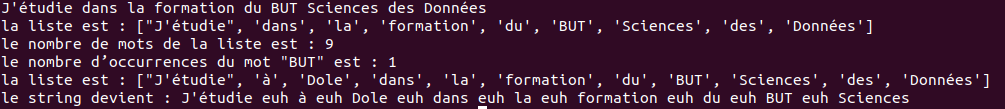
\includegraphics[scale = 0.4]{chapitre2/figures/string2.png}
\end{figure}


\textbf{2$\diamondsuit$-}
Complétez le programme suivant de façon à partir d'un string obtenu

\begin{enumerate}
    \item mettez le string en majuscule (aide : upper()\footnote{\url{https://www.geeksforgeeks.org/python-string-upper/}})
    \item remplacez les "euh" par un espace " " (aide : replace() )
    \item afficher si le string contient le mot "DOLE" (aide : rfind())
\end{enumerate}

Puis, recréez une liste à partir de ce string et affichez là en minuscule.

\textbf{(Optionnel)3$\diamondsuit~\diamondsuit~\diamondsuit$-}
Modifier la comparaison avec "DOLE" de façon à ce qu'elle soit insensible à la case.

\end{tcolorbox}



\subsection{Tuples}

\textbf{Les éléments d'un tuple sont ordonnés, immuables et peuvent être dupliqués.}
En mathématiques, on parle de p-uplets, avec $p$ ne nombre d'éléments \url{https://python-reference.readthedocs.io/en/latest/docs/tuple/}. 


Ouvrez un éditeur de texte et écrivez :

\lstinputlisting[language = python]{chapitre2/codes/tuple.py}

La sortie écran que vous devez obtenir est la suivante : 

\begin{figure}[H]
    \centering
    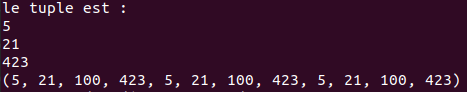
\includegraphics[scale = 0.5]{chapitre2/figures/tuple.png}
\end{figure}


\begin{tcolorbox}[lefttitle=2cm, colframe=gray!75!black, title= \textbf{Exercices}]
\textbf{1$\diamondsuit$-}
Complétez le programme précédent de façon à fournir :

\begin{enumerate}
    \item la somme des dépenses
    \item la dépense la plus importante
    \item la dépense la moins importante
    \item le nombre de loyers payés (montant 423)
    \item le nombre de dépenses
    \item la moyenne des dépenses
    \item la somme des dépenses
\end{enumerate}

L'affichage termianl obtenu devrait être le suivant :

\begin{figure}[H]
    \centering
    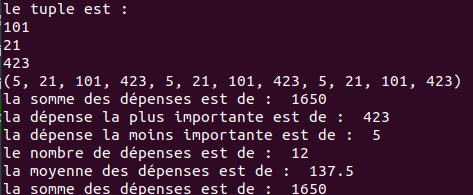
\includegraphics[scale = 0.6]{chapitre2/figures/tuple2.png}
\end{figure}

Aide : \url{https://python-reference.readthedocs.io/en/latest/docs/tuple/}

\end{tcolorbox}


\begin{tcolorbox}[lefttitle=2cm, colframe=gray!75!blue, title= \textbf{Tip for Code 3 : psychologie d'un tuple}]

Les tuples étant non modifiables, que se passe-t-il alors avec un tuple contenant des objets modifiables comme des listes ? 
\begin{figure}[H]
    \begin{minipage}[c]{0.53\textwidth}
Analyse du code suivant code suivant :
\lstinputlisting[language = python]{chapitre2/codes/tupleAvecListe2.py}

    \end{minipage}\hfill
    \begin{minipage}[c]{0.45\textwidth}

Il existe deux grands types de copie :
\begin{itemize}
    \item La copie par valeur recrée un objet identique. Deux objets d'adresse différente mais de valeur identique sont créés.
    \item La copie par référence copie l'adresse (ou référence) de l'objet. Il n'existe donc qu'un seul objet.
\end{itemize}

    \begin{center}
    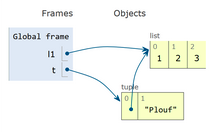
\includegraphics[scale=0.7]{chapitre2/figures/memoire.png}    
    \end{center}
    
    
La liste l1 pointe vers le même objet que l'élément du tuple d'indice 0. C'est une copie par référence (même adresse).
Donc, Dans notre cas, le premier élément du tuple pointe vers une liste modifiable. 

    \end{minipage}
\end{figure}

\end{tcolorbox}




\subsection{Sets}

\textbf{Les éléments de l'ensemble sont non ordonnés, non modifiables et n'autorisent pas les valeurs en double.}

Pour manipuler un ensemble, ouvrez un éditeur de texte et
écrivez :

\lstinputlisting[language = python]{chapitre2/codes/ens3.py}

La sortie écran obtenue est la suivante : 

\begin{figure}[H]
    \centering
    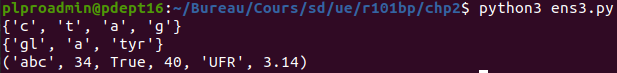
\includegraphics[scale = 0.7]{chapitre2/figures/ens3.png}
\end{figure}

\begin{tcolorbox}[lefttitle=2cm, colframe=gray!75!blue, title= \textbf{Tip for Code 4 : "\textit{Les duplications dans les ensembles}"}]

Les ensembles ne peuvent pas comporter deux éléments ayant la même valeur.
Les valeurs en double seront ignorées.
Le programme suivant :
\lstinputlisting[language = python]{chapitre2/codes/ens.py}
donnera la sortie écran suivante :


\begin{figure}[H]
    \centering
    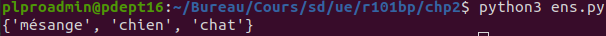
\includegraphics[scale = 0.7]{chapitre2/figures/ens.png}
\end{figure}

A votre avis, que donnera le programme suivant ?

\lstinputlisting[language = python]{chapitre2/codes/ens2.py}




\end{tcolorbox}


\begin{tcolorbox}[lefttitle=2cm, colframe=gray!75!black, title= \textbf{Exercice}]
\textbf{1$\diamondsuit$-}
A l'aide du programme précédent et de votre ordinateur, complétez le tableau suivant


\textbf{set}

\begin{tabular}{|l|c|}
    \hline   Instructions &  ~~~~~~~~~~~~~~~~~~~~~~~~~~~~~~~~~~~~~~~~~~~~Sortie écran ~~~~~~~~~~~~~~~~~~~~~~~~~~~~~~~~~~~~~~~~~~~~\\\hline
     $s = \{3, 4, "Plouf", (1, 3)\}$ & \\
     $print(s)$ &  \\\hline
      $s2 = \{3.14, [1, 2]\}$ & \\
     $print(s)$ &  \\\hline
       $print((set((2, 2, 2, 1))))$& \\\hline
      $s3 = set("BUT SD S1")$ &  \\ 
       $print(s3)$&\\\hline
      $s3.add(1)$ &  \\ 
       $print(s3)$&\\\hline
      $s3.discard('1')$ &  \\ 
       $print(s3)$&\\\hline
      $s3.discard('t')$ & \\ 
       $print(s3)$&\\\hline
      $print(s3.intersection(s))$&\\\hline
\end{tabular}


\end{tcolorbox}


\begin{tcolorbox}[lefttitle=2cm, colframe=gray!75!blue, title= \textbf{Tip for Code 5 : Etre ou ne pas être (hashable)}]

Commençons avec un rappel de vocabulaire :

\textbf{Un objet mutable} est ainsi un objet qui peut être modifié, dont on peut changer les propriétés une fois qu’il a été 
défini.\footnote{\url{https://docs.python.org/3/glossary.html\#term-mutable}}


A l'inverse, \textbf{un objet hashable} ne peut être modifié une fois qu’il a été 
défini.\footnote{\url{https://docs.python.org/3/glossary.html\#term-hashable}}

Les sets ne peuvent contenir que des objets hachables. Avoir des objets hashables optimise l'accès à chaque élément du set. Les objets hachables sont les chaînes de caractères, les tuples, les entiers, les floats, les booléens et les frozensets. Les objets non hachables que l'on connait sont les listes, les sets et les dictionnaires. 

\end{tcolorbox}






\subsection{Dictionaires}


Les dictionnaires permettent de manipuler des structures complexes. \textbf{Les dictionnaires sont des collections non ordonnées d'objets}. Il s'agit d'objets correspondance (mapping objects en anglais) ou tableaux associatifs. En effet, dans un même dictionnaire chaque valeur d'objet est accessible par une clé.


Pour manipuler un ensemble, ouvrez un éditeur de texte et
écrivez :

\lstinputlisting[language = python]{chapitre2/codes/dict.py}

La sortie écran obtenue est la suivante : 

\begin{figure}[H]
    \centering
    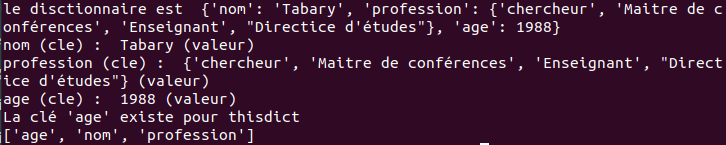
\includegraphics[scale = 0.7]{chapitre2/figures/dict.png}
\end{figure}


\begin{tcolorbox}[lefttitle=2cm, colframe=gray!75!black, title= \textbf{Exercice}]
\textbf{1$\diamondsuit$-}
Modifier le code précédent afin d'enlever la valeur enseignant chercheur au dictionnaire.

\textbf{2$\diamondsuit~\diamondsuit$-}
Rajouter le dictionnaire suivant au code

\begin{figure}[H]
    \centering
    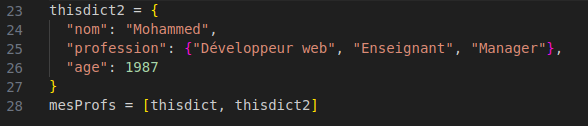
\includegraphics[scale = 0.7]{chapitre2/figures/dict2.png}
\end{figure}

\begin{itemize}
    \item affichez les noms de vos professeurs grâce à une boucle
    \item affichez l'ensemble des professions communes aux deux professeurs
\end{itemize}




\end{tcolorbox}


\subsection{Projets (optionnels)}


La recherche dichotomique prend en entrée une liste triée  \textit{T} et un élément \textit{v}.
Elle donne en résultat l'index, tel que \textit{T[index] = v}.
\subsubsection{Recherche simple}

On procède comme suit :
\begin{itemize}
    \item On compare v à chaque élément de la liste
    \item S’il est égal à v, on a fini
    \item Sinon, on prend l'élément suivant
    \item S’il est supérieur, on affiche l'information "pas d'éléments" sur le terminal
\end{itemize}

Donnez une preuve de terminaison, et la complexité de ce programme.


\textbf{Programmez un algorithme de recherche dichotomique.
}


\subsubsection{Recherche dichotomique}

On procède comme suit :
\begin{itemize}
    \item On compare v à l’élément du milieu de la liste.
    \item S’il est égal à v, on a fini.
    \item Sinon, s’il est inférieur, il faut chercher dans la première moitié de la liste. On retourne à l’étape 1 avec la liste réduite.
    \item S’il est supérieur, on fait de même avec la seconde moitié de la liste.
\end{itemize}

\textbf{Programmez un algorithme de recherche dichotomique.
}

Donnez une preuve de terminaison, et la complexité de ce programme.

\newpage

\subsection{Bilan (obligatoire)}



\makebox[0.75\textwidth]{Lors de ce TP, vous vous êtes arrêté à quel exercice ? \enspace\hrulefill}


\makebox[1\textwidth]{--------------------------------------------------Remplir le tableau--------------------------------------------------}

\textbf{Partie savoir faire}
\begin{itemize}
    \item Niveau 1 : Je n'ai pas su l'implémenter. C'est du charabiah pour moi. 
    \item Niveau 2 : J'ai lu le sujet. Les couleurs sont jolies. J'ai fini le premier exercice les yeux rivés sur mon clavier pour chercher les touches. Les erreurs de l'interpréteur me semblent incompréhensibles.
    \item Niveau 3 : J'ai pu avancer à la moitié du sujet, même si c'est difficile et que l'ordi est farceur (comme tous les ordis). Je prends beaucoup de temps à comprendre les erreurs du shell, mais j'y arrive !
    \item Niveau 4 : J'ai complété le TP avec aisance. La plupart des erreurs du shell me sont compréhensibles.
    \item Niveau 5 : J'ai complété le TP, exercices optionnels compris ! J'ai une grande agilité\footnote{agilité $\rightarrow$ ne pas utiliser la souris en codant} quand je code. 
\end{itemize}


\textbf{Partie savoir être}
\begin{itemize}
    \item Niveau 1 :  Pour finir au plus vite, j'élabore des stratégies (copier directement la réponse ou chercher à camoufler le désintérêt : "Si je n'y arrive pas, c'est que le prof n'est pas venu assez vite me donner la solution"). 
    \item Niveau 2 : L'objectif est d'avoir la moyenne sans trop y laisser du temps ou de l'énergie. Je suis bien obligé de faire le TP, même si l'idée de me servir du pannel de ressources me semble saugrenue. Si c'est possible de récupérer la réponse (ou de suivre à côté d'un camarade\footnote{Mais si, c'est du travail d'équipe : il code et je le soutiens émotionnellement !}), alors je ne dirai pas non. 
    \item Niveau 3 : Je prends doucement mes marques. Je me suis servi de façon hésitante de plusieurs ressoures dispos (shell, camarades, enseignants, manuel, sites web, ou même canard\footnote{\url{https://fr.wikipedia.org/wiki/M\%C3\%A9thode_du_canard_en_plastique}}) en cherchant à comprendre leur réponse. J'aimerais un jour pouvoir développer  mes propres projets et il faut pour cela que je gagne en autonomie.
    \item Niveau 4 :   Je suis autonome dans l'utilisation des ressoures disponibles (shell, camarades, enseignants, manuel, sites web, ou même canard\footnotemark[7]). J'ai même un projet personnel en cours que j'aimerais finir.
    \item Niveau 5 : J'évolue avec aisance dans cet environnement ! Je  fais même partie dorénavant des ressoures dispos et  j'échange facilement sur ces notions. J'ai plusieurs projets informatiques personnels. 
\end{itemize}

\begin{table}[H]
    \centering
    \begin{tabular}{|c|c|c|} \hline
        \textbf{Notions} & \textbf{Niveau atteint} (de 1 à 5) \textbf{Savoir faire}  & \textbf{Niveau atteint} (de 1 à 5) \textbf{Savoir être}\\\hline
        Liste & & \\\hline
        Tuple &&\\\hline
        Set &&\\\hline
        Dictionnaire &&\\\hline
        Respect des règles de bon codage && \\\hline
    \end{tabular}
\end{table}




\newpage
\section{TP3 : Lecture / écriture de fichier}

Un DataFrame est une structure de données étiquetée à deux dimensions avec des colonnes de types potentiellement différents. Un DataFrame peut-être une feuille de calcul, une table SQL ou un dictionnaire d'objets de série.

Ce TP vous invite à manipuler des dataframe à partir de fichiers externes.

\subsection{Fichiers de type texte (.txt)}




Pour manipuler un fichier texte, copiez/collez le fichier texte "bilbo1.txt" dans le même fichier que le progromme et écrivez ce programme dans un éditeur de texte :

\lstinputlisting[language = python]{chapitre3/codes/texte.py}

La sortie écran obtenue est la suivante : 

\begin{figure}[H]
    \centering
    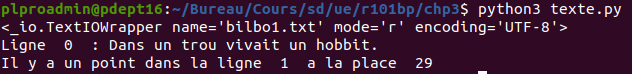
\includegraphics[scale = 0.5]{chapitre3/figures/texte.png}
\end{figure}

On retrouve les méthodes de manipulation des strings (chaînes de caractère), vues dans le chapitre précédent, et détaillées dans le manuel
\footnote{\url{https://www.w3schools.com/python/python_ref_string.asp}}.

\begin{tcolorbox}[lefttitle=2cm, colframe=gray!75!blue, title= \textbf{Tip for Code 1 : "\textit{les Droits}"}]

Les droits sur le fichier manipuler sont déclinés par les lettres suivantes :

r, pour une ouverture en lecture (READ).

w, pour une ouverture en écriture (WRITE), à chaque ouverture le contenu du fichier est écrasé. Si le fichier n'existe pas python le crée.

a, pour une ouverture en mode ajout à la fin du fichier (APPEND). Si le fichier n'existe pas python le crée.

b, pour une ouverture en mode binaire.

t, pour une ouverture en mode texte.

x, crée un nouveau fichier et l'ouvre pour écriture


\end{tcolorbox}


\begin{tcolorbox}[lefttitle=2cm, colframe=gray!50!red, title= \textbf{ WARNING}]
\textbf{Tout fichier ouvert (avec open) doit être fermé  (avec close).}

Tout oubli à ce sujet, vaudra une division par 2 de la note de l'exercice en question.
\end{tcolorbox}


\begin{tcolorbox}[lefttitle=2cm, colframe=gray!75!black, title= \textbf{Exercices}]
\textbf{1$\diamondsuit$-}
Le premier exercice vous invite à manipuler des fichiers textes.

\begin{enumerate}
    \item Mettre les fichiers textes "bilbo1.txt", "bilbo2.txt" et "bilbo3.txt" dans un dossier intitulé "fichiersTexte" dans le même dossier que votre programme. 
    \item Créer un nouveau fichier texte vide, appelé "bilbo.txt".
    \item Concaténer les 3 fichiers en un nouveau fichier "blibo.txt", lui-même placé dans le dossier "fichiersTexte".
\end{enumerate}

\textbf{2$\diamondsuit$-}
Modifier votre code de façon à créer le fichier texte "bilbo.txt" s'il n'est pas existant.

\textbf{3$\diamondsuit~\diamondsuit$-}
Modifier votre code afin de changer le mot "hobbit" par "Periannath" (langue elfique).

\textbf{(Optionnel)4$\diamondsuit~\diamondsuit$-}
Modifier votre programme afin d'intégrer, si ce n'est pas déjà fait, la librairie de gestion des fichiers "import os"\footnote{\url{https://docs.python.org/fr/3/library/os.html}} pour importer l'adresse du fichier courant. 

\textbf{(Optionnel)5$\diamondsuit~\diamondsuit~\diamondsuit$-}
Créer un programme qui prend en entrée un dossier. Et en sortie, ce programme affiche la hiérarchie des éléments au sein de ce dossier, avec le type de ces éléments (fichier, dossier, executable, ou autres).

\end{tcolorbox}

\subsection{Les fichiers csv}

Un fichier CSV (Comma-separated values) est un type de fichier associé à Excel. Plutôt que de stocker les informations en colonnes, les fichiers CSV les stockent en les séparant par des points-virgules.

Le csv utilié lors de ce TP est disponible sur le site de l'INSEE\footnote{\url{https://www.insee.fr/fr/statistiques/2540004?sommaire=4767262\#consulter}}
sous le lien : Fichier allégé par département depuis 2000. 


\begin{figure}[H]
    \centering
    
\includegraphics[scale = 0.5]{chapitre3/figures/csvINSEE.png}
\end{figure}

Télécharger l'archive dans un dossier intitulé "fichiersCSV", dans le même répertoire que celui contenant votre dossier "fichiersTexte".


Ensuite, copier le programme suivant :

\lstinputlisting[language = python]{chapitre3/codes/EcritureLecturecsv.py}

La sortie écran obtenue est la suivante : 

\begin{figure}[H]
    \centering
    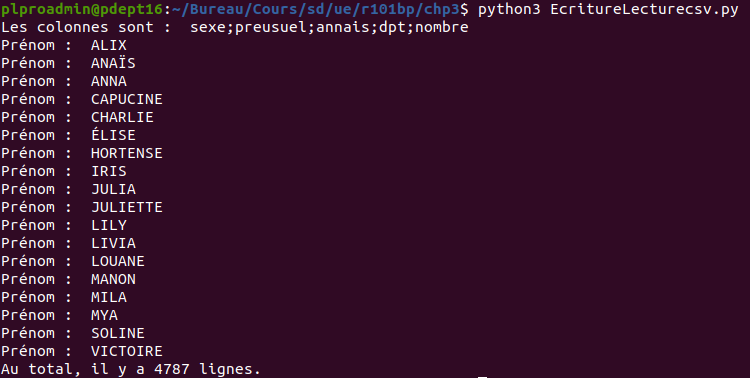
\includegraphics[scale = 0.5]{chapitre3/figures/csvex.png}
\end{figure}


\begin{tcolorbox}[lefttitle=2cm, colframe=gray!75!black, title= \textbf{Exercices}]
\textbf{1$\diamondsuit$-}
Le premier exercice vous invite à manipuler le programme précédent de façon à :

\begin{enumerate}
    \item Enumérer les prénoms féminins de 2021 qui apparaissent -cette fois- moins de 5 fois 
    \item Ecrire le résultat dans un fichier .txt, avec la mention "prénom rare" à côté, si le prénom apparaît moins de 4 fois.
\end{enumerate}

\textbf{(Optionnel) 2$\diamondsuit$-} Concaténer les deux cvs du Jura (39) et du Doubs (25) en un seul csv

\textbf{(Optionnel)3$\diamondsuit$-} Pourquoi vous ne devez pas appeler votre fichier python csv.py ?
\end{tcolorbox}

\subsection{Fichiers de type xlsx}

Le fichier xlsx est l'extension par défaut des fichiers créés avec la version 2007 du logiciel Excel.

Le xlsx utilié lors de ce TP est disponible sur le site de l'INSEE\footnote{\url{https://www.insee.fr/fr/statistiques/6011070?sommaire=6011075}}
sous le lien : France hors Mayotte. 


\begin{figure}[H]
    \centering
    
\includegraphics[scale = 0.5]{chapitre3/figures/xlsxTl.png}
\end{figure}

Télécharger le fichier dans un dossier intitulé "fichiersXLSX", dans le même répertoire que celui contenant vos dossiers "fichiersTexte" et "fichiersCSV".

Ensuite, copier le programme suivant :

\lstinputlisting[language = python]{chapitre3/codes/EcritureLecturexlsx.py}


\begin{tcolorbox}[lefttitle=2cm, colframe=gray!75!black, title= \textbf{Exercice}]
Pourquoi il est déconseillé d'écrire L 22 : " if x.startswith('Dol') and type(x) == str:"  ?
\vspace{2cm}
\end{tcolorbox}



La sortie écran obtenue est la suivante : 

\begin{figure}[H]
    \centering
    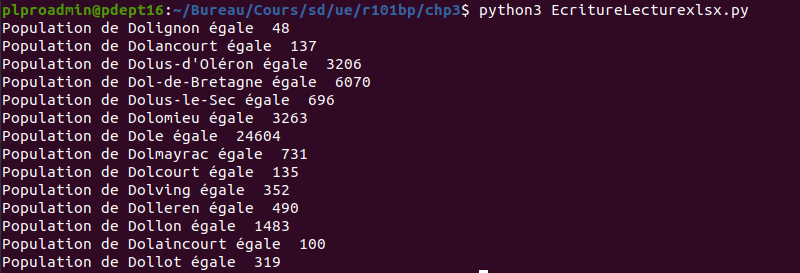
\includegraphics[scale = 0.5]{chapitre3/figures/xlsxCE.png}
\end{figure}

On retrouve les méthodes de manipulation des strings (chaînes de caractère), vues dans le chapitre précédent, et détaillées dans le manuel
\footnote{\url{https://www.w3schools.com/python/python_ref_string.asp}}.

De plus, on utilise la méthode enumerate \footnote{\url{https://docs.python.org/3/library/functions.html\#enumerate}} pour accéder aux index de la boucle (voir chapitre précédent). 

\begin{tcolorbox}[lefttitle=2cm, colframe=gray!75!blue, title= \textbf{Tip for Code 2 : "\textit{Panel Data}"}]


La bibliothèque logicielle open-source Pandas est spécifiquement conçue pour la manipulation et l’analyse de données en langage Python. Elle est à la fois performante, flexible et simple d’utilisation.

Grâce à Pandas, le langage Python permet enfin de charger, d’aligner, de manipuler ou encore de fusionner des données. Les performances sont particulièrement efficaces quand le code source back-end est écrit en C ou en Python.

Le manuel est disponible à cette adresse :
\url{https://pandas.pydata.org/docs/reference/api/pandas.ExcelFile.html}

\end{tcolorbox}




\begin{tcolorbox}[lefttitle=2cm, colframe=gray!75!black, title= \textbf{Exercices}]
\textbf{1$\diamondsuit$-}
Le premier exercice vous invite à manipuler le programme précédent de façon à :
Afficher sur le terminal la population totale des villes commençant par "Dol"

    
\textbf{(Optionnel)2$\diamondsuit~\diamondsuit$-} 
On s'intéresse en suite aux communes dont la commune pôle est Mièges (Mièges comprise), dans la feuille "Communes associées ou déléguées".
Créer un fichier texte contenant :
\begin{enumerate}
    \item le nombre de ces communes
    \item leur nom, leur population municipale et leur population totale
    \item si leur population comptée à part est null, rajouter la mention "urbain"
    \item afficher la population totale
\end{enumerate}

    
\textbf{(Optionnel)3$\diamondsuit~\diamondsuit~\diamondsuit$-} 
Creer un nouveau fichier xlsx, de façon à avoir les colonnes de la feuille "Communes associées ou déléguées", avec le numéro de Canton (dans la feuille "Communes").

Vous rajouterez également une visualisation de la population de votre choix en utilisant la bibliothèque plot \footnote{\url{https://pandas.pydata.org/docs/user_guide/visualization.html}}.


\textbf{(Optionnel)4$\diamondsuit$-} Pourquoi vous ne devez pas appeler votre fichier python csv.py ?
\end{tcolorbox}


\subsection{Fichiers de type json }




\begin{tcolorbox}[lefttitle=2cm, colframe=gray!50!yellow, title= \textbf{ JSON}]
Le JavaScript Object Notation (JSON) est un format standard utilisé pour représenter des données structurées de façon semblable aux objets Javascript.
Un json est représenté par une liste de dictionnaires.

\begin{figure}[H]
    \centering
    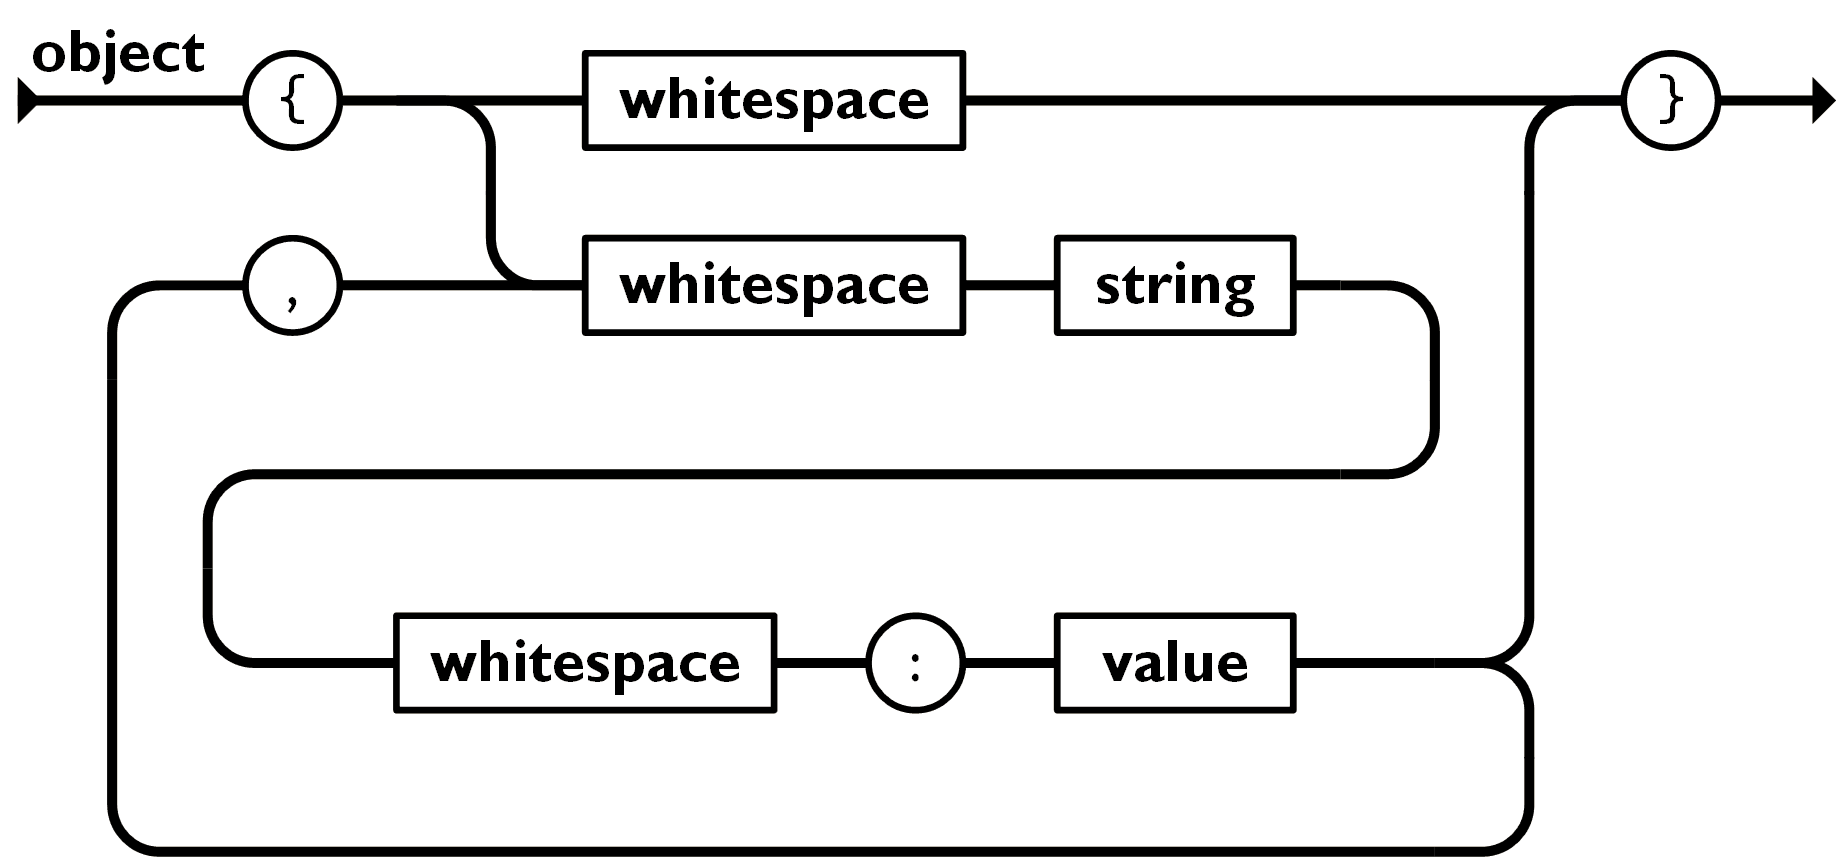
\includegraphics[scale = 0.5]{chapitre3/figures/jsonImg.png}
\end{figure}

\end{tcolorbox}


Pour cet exercice, copier le programme suivant : 
\lstinputlisting[language = python]{chapitre3/codes/EcritureLecturejson.py}

La sortie écran obtenue est la suivante : 

\begin{figure}[H]
    \centering
    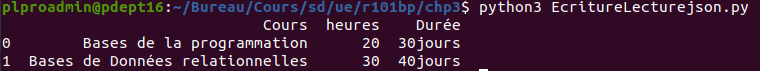
\includegraphics[scale = 0.5]{chapitre3/figures/json.png}
\end{figure}

\begin{tcolorbox}[lefttitle=2cm, colframe=gray!75!black, title= \textbf{Exercice}]
\textbf{1$\diamondsuit$-}
A partir du manuel\footnote{\url{https://pythonbasics.org/pandas-json/}} et du programme précédent, rajouter le numéro de semestre correspondant au cours et les notes de ces matières.

\end{tcolorbox}


\newpage

\subsection{Bilan (obligatoire)}



\makebox[0.75\textwidth]{Lors de ce TP, vous vous êtes arrêté à quel exercice ? \enspace\hrulefill}


\makebox[1\textwidth]{--------------------------------------------------Remplir le tableau--------------------------------------------------}

\textbf{Partie savoir faire}
\begin{itemize}
    \item Niveau 1 : Je n'ai pas su l'implémenter. C'est du charabiah pour moi. 
    \item Niveau 2 : J'ai lu le sujet. Les couleurs sont jolies. J'ai fini le premier exercice les yeux rivés sur mon clavier pour chercher les touches. Les erreurs de l'interpréteur me semblent incompréhensibles.
    \item Niveau 3 : J'ai pu avancer à la moitié du sujet, même si c'est difficile et que l'ordi est farceur (comme tous les ordis). Je prends beaucoup de temps à comprendre les erreurs du shell, mais j'y arrive !
    \item Niveau 4 : J'ai complété le TP avec aisance. La plupart des erreurs du shell me sont compréhensibles.
    \item Niveau 5 : J'ai complété le TP, exercices optionnels compris ! J'ai une grande agilité\footnote{agilité $\rightarrow$ ne pas utiliser la souris en codant} quand je code. 
\end{itemize}


\textbf{Partie savoir être}
\begin{itemize}
    \item Niveau 1 :  Pour finir au plus vite, j'élabore des stratégies (copier directement la réponse ou chercher à camoufler le désintérêt : "Si je n'y arrive pas, c'est que le prof n'est pas venu assez vite me donner la solution"). 
    \item Niveau 2 : L'objectif est d'avoir la moyenne sans trop y laisser du temps ou de l'énergie. Je suis bien obligé de faire le TP, même si l'idée de me servir du pannel de ressources me semble saugrenue. Si c'est possible de récupérer la réponse (ou de suivre à côté d'un camarade\footnote{Mais si, c'est du travail d'équipe : il code et je le soutiens émotionnellement !}), alors je ne dirai pas non. 
    \item Niveau 3 : Je prends doucement mes marques. Je me suis servi de façon hésitante de plusieurs ressoures dispos (shell, camarades, enseignants, manuel, sites web, ou même canard\footnote{\url{https://fr.wikipedia.org/wiki/M\%C3\%A9thode_du_canard_en_plastique}}) en cherchant à comprendre leur réponse. J'aimerais un jour pouvoir développer  mes propres projets et il faut pour cela que je gagne en autonomie.
    \item Niveau 4 :   Je suis autonome dans l'utilisation des ressoures disponibles (shell, camarades, enseignants, manuel, sites web, ou même canard\footnotemark[7]). J'ai même un projet personnel en cours que j'aimerais finir.
    \item Niveau 5 : J'évolue avec aisance dans cet environnement ! Je  fais même partie dorénavant des ressoures dispos et  j'échange facilement sur ces notions. J'ai plusieurs projets informatiques personnels. 
\end{itemize}

\begin{table}[H]
    \centering
    \begin{tabular}{|c|c|c|} \hline
        \textbf{Notions} & \textbf{Niveau atteint} (de 1 à 5) \textbf{Savoir faire}  & \textbf{Niveau atteint} (de 1 à 5) \textbf{Savoir être}\\\hline
        txt & & \\\hline
        csv &&\\\hline
        xlsx &&\\\hline
        json &&\\\hline
        Respect des règles de bon codage && \\\hline
    \end{tabular}
\end{table}





\newpage
\section{TP4 : Entraînement contrôle}

Ces exercices sont issus de \url{https://adventofcode.com/2015/day/1}.

\subsection{Exercice 1. Année 2015, jour 1}


Vous avez en entrée un fichier texte exo1.txt contenant des parenthèses.
En sortie, vous devrez afficher la valeur d'une variable sur votre terminal de commande.

\subsubsection{première partie}

--- Jour 1 : Pas tout à fait Lisp ---

Le Père Noël essaie de livrer des cadeaux dans un grand immeuble, mais il n'arrive pas à trouver le bon étage - les instructions qu'il a reçues sont un peu confuses. Il commence par le rez-de-chaussée (étage 0) et suit les instructions un caractère à la fois.

Une parenthèse ouvrante, (, signifie qu'il doit monter d'un étage, et une parenthèse fermante, ), signifie qu'il doit descendre d'un étage.

L'immeuble est très haut et le sous-sol est très profond ; il ne trouvera jamais l'étage supérieur ni l'étage inférieur.

Par exemple, (()) et ()()) :

    (()) et ()() donnent tous deux l'étage 0.

    ((( et (()((()( donnent tous deux l'étage 3.
    
    ))((((( donnent également l'étage 3.
    
    ()) et ))() donnent tous deux l'étage -1 (le premier niveau du sous-sol).
    
    ))) et )())()) donnent tous deux l'étage -3.

\textbf{A quel étage les instructions conduisent-elles le Père Noël ?}

\subsubsection{seconde partie}

Maintenant, avec les mêmes instructions, trouvez la position du premier personnage qui le fait entrer dans le sous-sol (étage -1). Le premier caractère dans les instructions a la position 1, le deuxième caractère a la position 2, et ainsi de suite.

Par exemple :

    ) le fait entrer dans le sous-sol à la position du caractère 1.
    
    ()()) le fait entrer dans le sous-sol à la position 5.
    
\textbf{    Quelle est la position du caractère qui fait entrer le Père Noël en premier dans la cave ?
}    

\subsection{Exercice 2. Année 2015, jour 2}

Vous avez en entrée un fichier texte exo2.txt contenant les données $a \times b \times c$ avec a,b et c des nombres.
En sortie, vous devrez afficher la valeur d'une variable sur votre terminal de commande.


\subsubsection{première partie}

--- Jour 2 : On m'a dit qu'il n'y aurait pas de maths...

Les lutins sont à court de papier d'emballage et doivent donc passer une commande pour en obtenir d'autres. Ils ont une liste des dimensions (longueur l, largeur w, et hauteur h) de chaque cadeau, et ne veulent commander que la quantité exacte dont ils ont besoin.

Heureusement, chaque cadeau est une boîte (un prisme rectangulaire droit parfait), ce qui facilite le calcul du papier d'emballage nécessaire pour chaque cadeau : trouver la surface de la boîte, qui est 2*l*w + 2*w*h + 2*h*l. Les lutins ont également besoin d'un peu de papier supplémentaire pour chaque cadeau : la surface du plus petit côté.

C'est l'aire du plus petit côté :

    Un cadeau de dimensions 2x3x4 nécessite 2*6 + 2*12 + 2*8 = 52 mètres carrés de papier d'emballage plus 6 mètres carrés de mou, soit un total de 58 mètres carrés.

    Un cadeau de dimensions 1x1x10 nécessite 2*1 + 2*10 + 2*10 = 42 mètres carrés de papier d'emballage plus 1 mètre carré de jeu, pour un total de 43 mètres carrés.

Tous les nombres de la liste des lutins sont exprimés en pieds. 

\textbf{Combien de mètres carrés de papier d'emballage doivent-ils commander ?}

\subsubsection{seconde partie}


Les lutins sont également à court de ruban. Les rubans étant tous de la même largeur, ils n'ont qu'à se préoccuper de la longueur qu'ils doivent commander, qu'ils voudraient encore une fois exacte.

Le ruban nécessaire pour emballer un cadeau correspond à la distance la plus courte autour de ses côtés, ou au plus petit périmètre d'une face. Chaque cadeau a également besoin d'un nœud fait de ruban ; le nombre de pieds de ruban requis pour un nœud parfait est égal au volume en pieds cubes du cadeau. Ne demandez pas comment ils font le nœud, ils ne vous le diront jamais.

Voici un exemple :

    Un cadeau de dimensions 2x3x4 nécessite 2+2+3+3 = 10 pieds de ruban pour envelopper le cadeau, plus 2*3*4 = 24 pieds de ruban pour le nœud, soit un total de 34 pieds.
    
    Un cadeau aux dimensions 1x1x10 nécessite 1+1+1+1 = 4 pieds de ruban pour envelopper le cadeau plus 1*1*10 = 10 pieds de ruban pour le nœud, soit un total de 14 pieds.

\textbf{Combien de mètres de ruban doivent-ils commander au total ?}


\subsection{Exercice 3. Année 2015, jour 3}


Vous avez en entrée un fichier texte exo3.txt.
En sortie, vous devrez afficher la valeur d'une variable sur votre terminal de commande.

\subsubsection{première partie}

--- Jour 3 : Des maisons parfaitement sphériques dans le vide ---

Le Père Noël livre des cadeaux à une grille bidimensionnelle infinie de maisons.

Il commence par livrer un cadeau à la maison située à son point de départ, puis un elfe du pôle Nord l'appelle par radio pour lui dire où se déplacer ensuite. Les déplacements se font toujours exactement d'une maison vers le nord (\^), le sud (v), l'est (>) ou l'ouest (<). Après chaque déplacement, il livre un autre cadeau à la maison de son nouvel emplacement.

Cependant, le lutin qui se trouve au pôle Nord a bu un peu trop de lait de poule, et ses indications sont donc un peu erronées, de sorte que le Père Noël finit par visiter certaines maisons plus d'une fois. \textbf{Combien de maisons reçoivent au moins un cadeau ?}

Par exemple :

    > livre des cadeaux à 2 maisons : l'une au point de départ, l'autre à l'est.
    
     	\textasciicircum >v< livre des cadeaux à 4 maisons dans un carré, dont deux fois à la maison située à son emplacement de départ/arrivée.
    
     	\textasciicircum v 	\textasciicircum v 	\textasciicircum v 	\textasciicircum v 	\textasciicircum v livre un tas de cadeaux à des enfants très chanceux dans seulement 2 maisons.


\subsubsection{seconde partie}
L'année suivante, pour accélérer le processus, le Père Noël crée une version robotisée de lui-même, Robo-Santa, pour livrer les cadeaux avec lui.

Le Père Noël et Robo-Santa commencent au même endroit (ils livrent deux cadeaux à la même maison de départ), puis se déplacent à tour de rôle en fonction des instructions du lutin, qui lit dans le lait de poule le même scénario que l'année précédente.

\textbf{Cette année, combien de maisons recevront au moins un cadeau ?}

Par exemple :

     	\textasciicircum v livre des cadeaux à 3 maisons, parce que le Père Noël va au nord et que Robo-Santa va au sud.
    
     	\textasciicircum >v< livre maintenant des cadeaux à 3 maisons, et le Père Noël et Robo-Santa reviennent à leur point de départ.
    
     	\textasciicircum v 	\textasciicircum v 	\textasciicircum v 	\textasciicircum v livre maintenant des cadeaux à 11 maisons, le Père Noël allant dans une direction et Robo-Santa dans l'autre.


\subsection{Exercice 4. Année 2015, jour 5}

Vous avez en entrée un fichier texte exo4.txt.
En sortie, vous devrez afficher la valeur d'une variable sur votre terminal de commande.

\subsubsection{première partie}

      --- Jour 5 : Il n'a pas de stagiaires pour cela ? ---

Le Père Noël a besoin d'aide pour déterminer quelles chaînes de son fichier texte sont bonnes ou fausses.

Une chaîne de caractères bonne est une chaîne qui possède toutes les propriétés suivantes :

    Elle contient au moins trois voyelles (aeiou uniquement), comme aei, xazegov, ou aeiouaeiouaeiou.
    
    Elle contient au moins une lettre qui apparaît deux fois de suite, comme xx, abcdde (dd), ou aabbccdd (aa, bb, cc, ou dd).
    Elle ne contient pas les chaînes ab, cd, pq ou xy, même si elles font partie de l'une des autres exigences.

Par exemple :

    ugknbfddgicrmopn est bonne parce qu'elle contient au moins trois voyelles (u...i...o...), une lettre double (...dd...), et aucune des sous-chaînes interdites.
    aaa est bonne parce qu'elle contient au moins trois voyelles et une lettre double, même si les lettres utilisées par les différentes règles se chevauchent.
    
    jchzalrnumimnmhp est fausse car elle n'a pas de lettre double.
    
    haegwjzuvuyypxyu est fausse car elle contient la chaîne xy.
    
    dvszwmarrgswjxmb est fausse car elle ne contient qu'une seule voyelle.

\textbf{Combien de chaînes sont bonnes ?}

\subsubsection{seconde partie}
Conscient de son erreur, le Père Noël a adopté un meilleur modèle pour déterminer si une ficelle est bonne ou fausse. Aucune des anciennes règles ne s'applique, car elles sont toutes clairement ridicules.

Désormais, une chaîne de caractères bonne est une chaîne qui possède toutes les propriétés suivantes :

    Elle contient une paire de deux lettres quelconques qui apparaissent au moins deux fois dans la chaîne sans se chevaucher, comme xyxy (xy) ou aabcdefgaa (aa), mais pas comme aaa (aa, mais elle se chevauche).
    Elle contient au moins une lettre qui se répète avec exactement une lettre entre elles, comme xyx, abcdefeghi (efe), ou même aaa.

Par exemple :

    qjhvhtzxzqqjkmpb est bonne parce qu'elle contient une paire qui apparaît deux fois (qj) et une lettre qui se répète avec exactement une lettre entre elles (zxz).

    xxyxx est bonne parce qu'elle contient une paire qui apparaît deux fois et une lettre qui se répète avec une lettre entre les deux, même si les lettres utilisées par chaque règle se chevauchent.
    
    uurcxstgmygtbstg est fausse car elle a une paire (tg) mais pas de répétition avec une seule lettre entre les deux.
    
    ieodomkazucvgmuy est fausse parce qu'elle contient une lettre répétée avec une lettre entre les deux (odo), mais pas de paire apparaissant deux fois.

\textbf{Combien de chaînes sont bonnes selon ces nouvelles règles ?}


\newpage
\section{Corrections}
\subsection{TP 1}

\textbf{Sortie terminal}
\lstinputlisting[language = python]{chapitre1/codes/second.py}

\textbf{Entrée utilisateur}
\lstinputlisting[language = python]{chapitre1/codes/entree2.py}

\textbf{Boucle for}

\lstinputlisting[language = python]{chapitre1/codes/tab2.py}

\textbf{Boucle tant que}

\lstinputlisting[language = python]{chapitre1/codes/while2.py}


\textbf{Juste prix}

\lstinputlisting[language = python]{chapitre1/codes/justePrix.py}

\subsection{TP 2}

\textbf{liste}

\lstinputlisting[language = python]{chapitre2/codes/liste2.py}

\textbf{string}

\lstinputlisting[language = python]{chapitre2/codes/string2.py}

\textbf{tuple}

\lstinputlisting[language = python]{chapitre2/codes/tuple.py}

\textbf{set}

\begin{tabular}{|l|c|}
    \hline   Instructions &  ~~~~~~~~~~~~~~~~~~~~~~Sortie écran ~~~~~~~~~~~~~~~~~~~~~~\\\hline
     $s = \{3, 4, "Plouf", (1, 3)\}$ & $\{'Plouf',(1, 3), 3, 4\}$ \\
     $print(s)$ &  \\\hline
      $s2 = \{3.14, [1, 2]\}$ & Erreur : liste non hashable\\
     $print(s)$ &  \\\hline
       $print((set((2, 2, 2, 1))))$& $\{1, 2\}$\\\hline
      $s3 = set("BUT SD S1")$ & $\{'T', 'D', 'B', 'S', '~', '1', 'U'\}$ \\ 
       $print(s3)$&\\\hline
      $s3.add(1)$ & $\{1, 'T', 'D', 'B', 'S', '~', 'U', '1'\}$ \\ 
       $print(s3)$&\\\hline
      $s3.discard('1')$ & $\{1, 'T', 'D', 'B', 'S', '~',  'U'\}$ \\ 
       $print(s3)$&\\\hline
      $s3.discard('t')$ & $\{1, 'T', 'D', 'B', 'S', '~',  'U'\}$ \\ 
       $print(s3)$&\\\hline
      $print(s3.intersection(s))$& $set()$  \\\hline
\end{tabular}


\textbf{dictionnaires}
\lstinputlisting[language = python]{chapitre2/codes/dict2.py}

\textbf{projet}
\lstinputlisting[language = python]{chapitre2/codes/listeTriee.py}
\subsection{TP 3}

\textbf{avec un fichier texte}

\lstinputlisting[language = python]{chapitre3/codes/texte2.py}

\subsection{TP 4}

La réponse à l'exo1, première partie, est 232.
La réponse à l'exo1, seconde partie, est 1783.

La réponse à l'exo2, première partie, est 1598415.
La réponse à l'exo2, seconde partie, est 3812909.


La réponse à l'exo3, première partie, est 2592.
La réponse à l'exo3, seconde partie, est 2360.


La réponse à l'exo4, première partie, est 238.
La réponse à l'exo4, seconde partie, est 2360.

%%%%%%%%%%%%%%%%%%%%%%%%%%%%%%%%%%%%%%%%%%%%%%%%%%%%%%%%%%%%%%%%%%
%Complete the assignment now
\end{document}

%%%%%%%%%%%%%%%%%%%%%%%%%%%%%%%%%%%%%%%%%%%%%%%%%%%%%%%%%%%%%%%%%%
%%%%%%%%%%%%%%%%%%%%%%%%%%%%%%%%%%%%%%%%%%%%%%%%%%%%%%%%%%%%%%%%%%
